\documentclass[]{book}
\usepackage{lmodern}
\usepackage{amssymb,amsmath}
\usepackage{ifxetex,ifluatex}
\usepackage{fixltx2e} % provides \textsubscript
\ifnum 0\ifxetex 1\fi\ifluatex 1\fi=0 % if pdftex
  \usepackage[T1]{fontenc}
  \usepackage[utf8]{inputenc}
\else % if luatex or xelatex
  \ifxetex
    \usepackage{mathspec}
  \else
    \usepackage{fontspec}
  \fi
  \defaultfontfeatures{Ligatures=TeX,Scale=MatchLowercase}
\fi
% use upquote if available, for straight quotes in verbatim environments
\IfFileExists{upquote.sty}{\usepackage{upquote}}{}
% use microtype if available
\IfFileExists{microtype.sty}{%
\usepackage[]{microtype}
\UseMicrotypeSet[protrusion]{basicmath} % disable protrusion for tt fonts
}{}
\PassOptionsToPackage{hyphens}{url} % url is loaded by hyperref
\usepackage[unicode=true]{hyperref}
\hypersetup{
            pdftitle={Inference in multivariate autoregressive process and its extensions},
            pdfauthor={Pierre Gloaguen},
            pdfborder={0 0 0},
            breaklinks=true}
\urlstyle{same}  % don't use monospace font for urls
\usepackage{natbib}
\bibliographystyle{apalike}
\usepackage{color}
\usepackage{fancyvrb}
\newcommand{\VerbBar}{|}
\newcommand{\VERB}{\Verb[commandchars=\\\{\}]}
\DefineVerbatimEnvironment{Highlighting}{Verbatim}{commandchars=\\\{\}}
% Add ',fontsize=\small' for more characters per line
\usepackage{framed}
\definecolor{shadecolor}{RGB}{248,248,248}
\newenvironment{Shaded}{\begin{snugshade}}{\end{snugshade}}
\newcommand{\KeywordTok}[1]{\textcolor[rgb]{0.13,0.29,0.53}{\textbf{#1}}}
\newcommand{\DataTypeTok}[1]{\textcolor[rgb]{0.13,0.29,0.53}{#1}}
\newcommand{\DecValTok}[1]{\textcolor[rgb]{0.00,0.00,0.81}{#1}}
\newcommand{\BaseNTok}[1]{\textcolor[rgb]{0.00,0.00,0.81}{#1}}
\newcommand{\FloatTok}[1]{\textcolor[rgb]{0.00,0.00,0.81}{#1}}
\newcommand{\ConstantTok}[1]{\textcolor[rgb]{0.00,0.00,0.00}{#1}}
\newcommand{\CharTok}[1]{\textcolor[rgb]{0.31,0.60,0.02}{#1}}
\newcommand{\SpecialCharTok}[1]{\textcolor[rgb]{0.00,0.00,0.00}{#1}}
\newcommand{\StringTok}[1]{\textcolor[rgb]{0.31,0.60,0.02}{#1}}
\newcommand{\VerbatimStringTok}[1]{\textcolor[rgb]{0.31,0.60,0.02}{#1}}
\newcommand{\SpecialStringTok}[1]{\textcolor[rgb]{0.31,0.60,0.02}{#1}}
\newcommand{\ImportTok}[1]{#1}
\newcommand{\CommentTok}[1]{\textcolor[rgb]{0.56,0.35,0.01}{\textit{#1}}}
\newcommand{\DocumentationTok}[1]{\textcolor[rgb]{0.56,0.35,0.01}{\textbf{\textit{#1}}}}
\newcommand{\AnnotationTok}[1]{\textcolor[rgb]{0.56,0.35,0.01}{\textbf{\textit{#1}}}}
\newcommand{\CommentVarTok}[1]{\textcolor[rgb]{0.56,0.35,0.01}{\textbf{\textit{#1}}}}
\newcommand{\OtherTok}[1]{\textcolor[rgb]{0.56,0.35,0.01}{#1}}
\newcommand{\FunctionTok}[1]{\textcolor[rgb]{0.00,0.00,0.00}{#1}}
\newcommand{\VariableTok}[1]{\textcolor[rgb]{0.00,0.00,0.00}{#1}}
\newcommand{\ControlFlowTok}[1]{\textcolor[rgb]{0.13,0.29,0.53}{\textbf{#1}}}
\newcommand{\OperatorTok}[1]{\textcolor[rgb]{0.81,0.36,0.00}{\textbf{#1}}}
\newcommand{\BuiltInTok}[1]{#1}
\newcommand{\ExtensionTok}[1]{#1}
\newcommand{\PreprocessorTok}[1]{\textcolor[rgb]{0.56,0.35,0.01}{\textit{#1}}}
\newcommand{\AttributeTok}[1]{\textcolor[rgb]{0.77,0.63,0.00}{#1}}
\newcommand{\RegionMarkerTok}[1]{#1}
\newcommand{\InformationTok}[1]{\textcolor[rgb]{0.56,0.35,0.01}{\textbf{\textit{#1}}}}
\newcommand{\WarningTok}[1]{\textcolor[rgb]{0.56,0.35,0.01}{\textbf{\textit{#1}}}}
\newcommand{\AlertTok}[1]{\textcolor[rgb]{0.94,0.16,0.16}{#1}}
\newcommand{\ErrorTok}[1]{\textcolor[rgb]{0.64,0.00,0.00}{\textbf{#1}}}
\newcommand{\NormalTok}[1]{#1}
\usepackage{longtable,booktabs}
% Fix footnotes in tables (requires footnote package)
\IfFileExists{footnote.sty}{\usepackage{footnote}\makesavenoteenv{long table}}{}
\usepackage{graphicx,grffile}
\makeatletter
\def\maxwidth{\ifdim\Gin@nat@width>\linewidth\linewidth\else\Gin@nat@width\fi}
\def\maxheight{\ifdim\Gin@nat@height>\textheight\textheight\else\Gin@nat@height\fi}
\makeatother
% Scale images if necessary, so that they will not overflow the page
% margins by default, and it is still possible to overwrite the defaults
% using explicit options in \includegraphics[width, height, ...]{}
\setkeys{Gin}{width=\maxwidth,height=\maxheight,keepaspectratio}
\IfFileExists{parskip.sty}{%
\usepackage{parskip}
}{% else
\setlength{\parindent}{0pt}
\setlength{\parskip}{6pt plus 2pt minus 1pt}
}
\setlength{\emergencystretch}{3em}  % prevent overfull lines
\providecommand{\tightlist}{%
  \setlength{\itemsep}{0pt}\setlength{\parskip}{0pt}}
\setcounter{secnumdepth}{5}
% Redefines (sub)paragraphs to behave more like sections
\ifx\paragraph\undefined\else
\let\oldparagraph\paragraph
\renewcommand{\paragraph}[1]{\oldparagraph{#1}\mbox{}}
\fi
\ifx\subparagraph\undefined\else
\let\oldsubparagraph\subparagraph
\renewcommand{\subparagraph}[1]{\oldsubparagraph{#1}\mbox{}}
\fi

% set default figure placement to htbp
\makeatletter
\def\fps@figure{htbp}
\makeatother

\usepackage{booktabs}

\title{Inference in multivariate autoregressive process and its extensions}
\author{Pierre Gloaguen}
\date{2020-06-19}

\begin{document}
\maketitle

{
\setcounter{tocdepth}{1}
\tableofcontents
}
\chapter{Introduction}\label{intro}

You can label chapter and section titles using \texttt{\{\#label\}}
after them, e.g., we can reference Chapter \ref{intro}. If you do not
manually label them, there will be automatic labels anyway, e.g.,
Chapter \ref{methods}.

Figures and tables with captions will be placed in \texttt{figure} and
\texttt{table} environments, respectively.

\begin{Shaded}
\begin{Highlighting}[]
\KeywordTok{par}\NormalTok{(}\DataTypeTok{mar =} \KeywordTok{c}\NormalTok{(}\DecValTok{4}\NormalTok{, }\DecValTok{4}\NormalTok{, .}\DecValTok{1}\NormalTok{, .}\DecValTok{1}\NormalTok{))}
\KeywordTok{plot}\NormalTok{(pressure, }\DataTypeTok{type =} \StringTok{'b'}\NormalTok{, }\DataTypeTok{pch =} \DecValTok{19}\NormalTok{)}
\end{Highlighting}
\end{Shaded}

\begin{figure}

{\centering 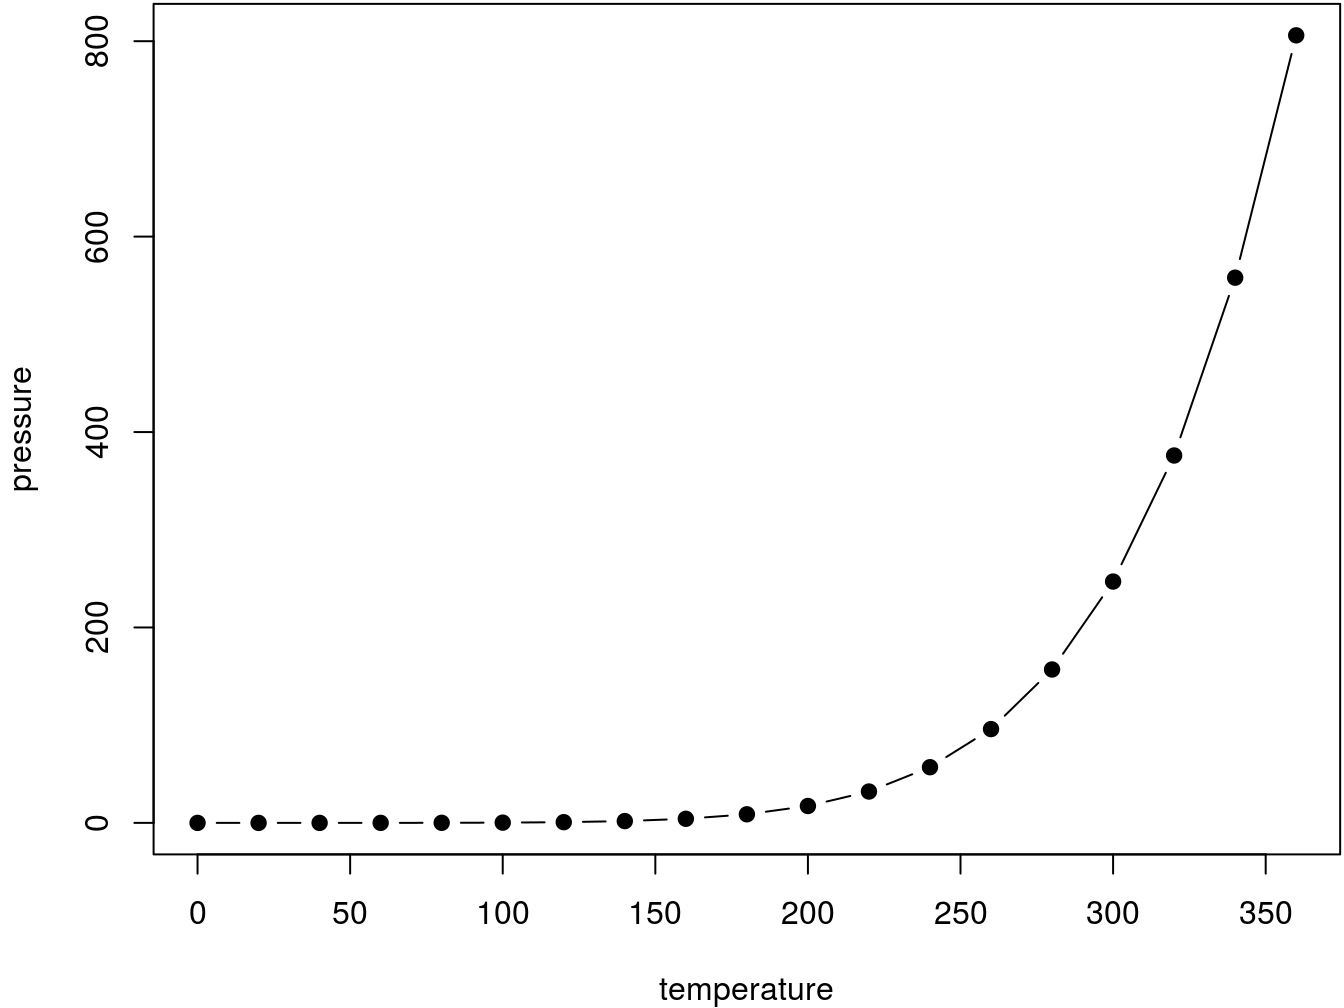
\includegraphics[width=0.8\linewidth]{topics_on_AR_model_files/figure-latex/nice-fig-1} 

}

\caption{Here is a nice figure!}\label{fig:nice-fig}
\end{figure}

Reference a figure by its code chunk label with the \texttt{fig:}
prefix, e.g., see Figure \ref{fig:nice-fig}. Similarly, you can
reference tables generated from \texttt{knitr::kable()}, e.g., see Table
\ref{tab:nice-tab}.

\begin{Shaded}
\begin{Highlighting}[]
\NormalTok{knitr}\OperatorTok{::}\KeywordTok{kable}\NormalTok{(}
  \KeywordTok{head}\NormalTok{(iris, }\DecValTok{20}\NormalTok{), }\DataTypeTok{caption =} \StringTok{'Here is a nice table!'}\NormalTok{,}
  \DataTypeTok{booktabs =} \OtherTok{TRUE}
\NormalTok{)}
\end{Highlighting}
\end{Shaded}

\begin{table}

\caption{\label{tab:nice-tab}Here is a nice table!}
\centering
\begin{tabular}[t]{rrrrl}
\toprule
Sepal.Length & Sepal.Width & Petal.Length & Petal.Width & Species\\
\midrule
5.1 & 3.5 & 1.4 & 0.2 & setosa\\
4.9 & 3.0 & 1.4 & 0.2 & setosa\\
4.7 & 3.2 & 1.3 & 0.2 & setosa\\
4.6 & 3.1 & 1.5 & 0.2 & setosa\\
5.0 & 3.6 & 1.4 & 0.2 & setosa\\
\addlinespace
5.4 & 3.9 & 1.7 & 0.4 & setosa\\
4.6 & 3.4 & 1.4 & 0.3 & setosa\\
5.0 & 3.4 & 1.5 & 0.2 & setosa\\
4.4 & 2.9 & 1.4 & 0.2 & setosa\\
4.9 & 3.1 & 1.5 & 0.1 & setosa\\
\addlinespace
5.4 & 3.7 & 1.5 & 0.2 & setosa\\
4.8 & 3.4 & 1.6 & 0.2 & setosa\\
4.8 & 3.0 & 1.4 & 0.1 & setosa\\
4.3 & 3.0 & 1.1 & 0.1 & setosa\\
5.8 & 4.0 & 1.2 & 0.2 & setosa\\
\addlinespace
5.7 & 4.4 & 1.5 & 0.4 & setosa\\
5.4 & 3.9 & 1.3 & 0.4 & setosa\\
5.1 & 3.5 & 1.4 & 0.3 & setosa\\
5.7 & 3.8 & 1.7 & 0.3 & setosa\\
5.1 & 3.8 & 1.5 & 0.3 & setosa\\
\bottomrule
\end{tabular}
\end{table}

You can write citations, too. For example, we are using the
\textbf{bookdown} package \citep{R-bookdown} in this sample book, which
was built on top of R Markdown and \textbf{knitr} \citep{xie2015}.

\chapter{Multivariate autoregressive model}\label{simpleAR}

In this chapter, we focus on the case where observations consist in a
multivariate time series \(y_0, \dots, y_n\) such that for any
\(0\leq t \leq n\), \(y_t \in \mathbb{R}^d\), we denote: \[y_t = 
\begin{pmatrix}
y_{t,1}\\
\vdots\\
y_{t, d}
\end{pmatrix}\]

\section{Model}\label{model}

We assume that these observations are realisations of random variables
\(Y_0,\dots, Y_n\) such that:

\begin{align}
Y_0 &\sim \chi_0(\cdot),\nonumber \\
Y_t &= m + \mathbf{A}Y_{t -1} + E_t,~1\leq t \leq n \label{eq:AR-simple}
\end{align}

where \(\chi_0\) is some probability distribution over \(\mathbb{R}^d\),
\(m\in\mathbb{R}^d\) and \(\mathbf{A}\in \mathcal{M}_{d\times d}\) are
parameters, \(E_t\) is a \(d-\)dimensionnal vector such that:

\begin{equation*}
E_t \overset{ind.}{\sim} \mathcal{N}\left(0, \mathbf{\Sigma}\right).
\end{equation*}

\section{Inference}\label{inference}

In this simple context, inference consists in finding the maximum
likelihood estimates of unknown
parameters\footnote{In the case where multiple time series are observed, unknown parameters for the initial distribution $\chi_0(\cdot)$ could be considered}
\(\hat{m}\), \(\hat{\mathbf{A}}\) and \(\mathbf{\Sigma}\).

Inference is straightforward here as we can recognize in
\eqref{eq:AR-simple} a multivariate linear model:
\[\mathbf{Y} = \mathbf{XB} + \mathbf{E},\] where

\begin{align*}
\mathbf{Y} &= 
\begin{pmatrix}
Y_1'\\
\vdots\\
Y_n'
\end{pmatrix} \in \mathcal{M}_{n \times d},\\
\mathbf{X} &= 
\begin{pmatrix}
1 & Y_0'\\
\vdots\\
1 & Y_{n-1}'
\end{pmatrix} \in \mathcal{M}_{n \times (d+1)},\\
\mathbf{B} &= 
\begin{pmatrix}
m'\\
A'
\end{pmatrix} \in \mathcal{M}_{(d + 1) \times d},\\
\mathbf{E} &= 
\begin{pmatrix}
E_1'\\
\vdots\\
E_n'
\end{pmatrix} \in \mathcal{M}_{n \times d}.
\end{align*}

Thus, \(\hat{m}\) and \(\hat{\mathbf{A}}\) can be obtained using the
classical estimate

\begin{equation}
\hat{\mathbf{B}} = \left(\mathbf{X'X}\right)^{-1}\mathbf{X}'\mathbf{Y}, \label{eq:AR-simple-B-hat}
\end{equation}

and \(\hat{\mathbf{\Sigma}}\) is then obtained classicaly as:

\begin{equation}
\hat{\mathbf{\Sigma}} = \frac{1}{n} \sum_{t = 1}^n \left(Y_t - \hat{m} - \hat{\mathbf{A}} Y_{t - 1}\right) \left(Y_t - \hat{m} - \hat{\mathbf{A}} Y_{t - 1}\right)' \label{eq:AR-simple-Sigma-hat}
\end{equation}

\chapter{Switching autoregressive
system}\label{switching-autoregressive-system}

In this chapter, we focus on a more complex system involving
autoregressive structure. We still focus on a time series
\(y_0, \dots, y_n\) of values in \(\mathbb{R}^d\). However, it is now
supposed that the time series dynamics could change through time,
according to an unobserved stochastic process in a discrete space. This
unobserved process might model different regimes of the dynamics (see
\citet{rabiner1989tutorial} for selected applications).

\section{Model}\label{model-1}

Taking the same notations and dimensions as in equation
\eqref{eq:AR-simple} We assume that these observations are realisations of
random variables \(Y_0,\dots, Y_n\) such that:

\begin{align*}
Z_0 &\sim \chi_{0, Z}(\cdot)\\
Z_t \vert Z_{t - 1} &\sim p(z_t \vert Z_{t - 1}) \\
Y_0 &\sim \chi_{0, Y}(\cdot \vert Z_0), \\
Y_t \vert Z_t &= m(Z_t) + \mathbf{A}(Z_t)Y_{t -1} + E_t,~1\leq t \leq n 
\end{align*}

where

\begin{itemize}
\tightlist
\item
  \(\left\lbrace Z_t \right\rbrace_{0\leq t \leq n}\) is an homogeneous
  Markov chain taking value on the finite space
  \(\mathbb{K} = \lbrace1,\dots, K \rbrace\), and of transition matrix
  denoted by \(\mathbf{P}\),
\item
  \(\lbrace m(k)\in\mathbb{R}^d,~\mathbf{A}(k)\in \mathcal{M}_{d\times d}\rbrace_{k = 1,\dots, K}\)
  are unknown parameters.
\item
  \(\chi_{0, Z}(\cdot)\) and \(\chi_{0, Y}(\cdot \vert Z_0)\) are some
  probability distributions over \(\mathbb{K}\) and \(\mathbb{R}^d\)
\item
  \(p(z_t\vert Z_{t-1})\) is the law of \(Z_t\) condtionnally to
  \(Z_{t - 1}\) (here the line of \(\mathbf{P}\) given by
  \(Z_{t - 1}\)).
\item
  \(E_t\) is a random vector such that:

  \begin{equation*}
  E_t \overset{ind.}{\sim} \mathcal{N}\left(0, \mathbf{\Sigma}\right).
  \end{equation*}

  where \(\mathbf{\Sigma}\) is \(d\times d\) covariance matrix.
\end{itemize}

In this context, the set of unknown parameters is given by
\[\theta = \left\lbrace \mathbf{P}, m(k),~\mathbf{A}(k), \mathbf{\Sigma}\right \rbrace_{k = 1,\dots, K}.\]

\section{Inference}\label{inference-1}

In this context, the inference task is twofold:

\begin{enumerate}
\def\labelenumi{\arabic{enumi}.}
\tightlist
\item
  Obtaining maximum likelihood estimate of \(\theta\);
\item
  Retracing the hidden sequence \(Z_0,\dots Z_n\) given the observations
  \(Y_{0:n}\).
\end{enumerate}

It is well known that these two tasks are indeed complementary. A common
way to solve these problems is the Expectation Maximization (EM)
algorithm \citep{dempster1977maximum}. The algorithm is shortly depicted
here.

\subsection{Comment about notations}\label{comment-about-notations}

In the following, we use the notation \(p\) for a generic probability
distribution. The law to which it refers is explicit through arguments.
For instance \(p(y_{0:n} \vert z_{0:n})\) is the p.d.f. of a Gaussian
vector, the random vector \(Y_{0:n}\vert Z_{0:n}\), and
\(p(z_t\vert z_{t - 1})\) is the law of the discrete random variable
\(Z_{t} \vert Z_{t - 1}\) evaluated at \(z_t\) and \(z_{t -1}\). In this
context,
\(p(z_t\vert z_{t - 1}) = \mathbb{P}(Z_t = z_t \vert \lbrace Z_{t-1} = z_{t -1}\rbrace.\)

\subsection{Likelihood}\label{likelihood}

A straightforward way to compute the likelihood in this model can be
obtained, just using the Markov properties of this model:

\begin{align}
L(\theta \vert y_{0:n}) &:= p(y_{0:n} \vert \theta) \nonumber \\
&= \sum_{z_{0:n}} p(y_{0:n}, z_{0:n}) \nonumber \\
&= \sum_{z_{0:n}} p(z_{0:n})p(y_{0:n}\vert z_{0:n}) \nonumber \\
&=  \sum_{z_{0:n}} p(z_0 \vert \theta) p(y_0\vert z_0, \theta) \prod_{t = 1}^n p(z_{t} \vert z_{t - 1}, \theta)p(y_{t}\vert y_{t -1}, z_{t}, \theta)  \label{eq:AR-HMM-likelihood}.
\end{align}

For a known \(\theta\), every term in \eqref{eq:AR-HMM-likelihood} can be
computed. However, in a general setting, there exists \(K^{n + 1}\)
possible sequences \(z_{0:n}\), which makes this direct computation
hardly feasible for any common values of \(n\).

\subsection{Complete log-likelihood}\label{complete-log-likelihood}

A workaround to find the maximum likelihood estimate is the EM
algorithm. In this context, we focus on a different function, the
\emph{complete log-likelihood}, i.e.~the likelihood of the
\emph{completed} observations (what we wish we could observe),
\((y_{0:n}, x_{0:n})\), we have that:

\begin{align}
\ell(\theta \vert y_{0:n}, z_{0:n}) :=& \log p(y_{0:n}, z_{0:n} \vert \theta) \nonumber \\
=& \log p(y_{0:n}, z_{0:n}) \nonumber \\
=& \log p(z_{0:n}) + \log p(y_{0:n}\vert z_{0:n}) \nonumber \\
=&  \log p(z_0 \vert \theta) + \log p(y_0\vert z_0, \theta) \nonumber \\ 
&+ \sum_{t = 1}^n \log p(z_{t} \vert z_{t - 1}, \theta) + \sum_{t = 1}^n \log p(y_{t}\vert y_{t -1}, z_{t}, \theta)  \label{eq:AR-HMM-complete-log-likelihood}.
\end{align}

For a given set of parameters, say \(\theta^{(0)}\), let's consider the
following function of \(\theta\)

\begin{align}
Q(\theta \vert \theta_0) &:= \mathbb{E}[\ell(\theta \vert Y_{0:n}, Z_{0:n}) \vert Y_{0:n} = y_{0:n}, \theta^{(0)}] \nonumber\\ 
&= \sum_{z_{0:n}} \ell(\theta \vert y_{0:n}, z_{0:n}) p(z_{0:n} \vert y_{0:n}, \theta^{(0)}) \text{d} z_{0:n} \nonumber \\
&= \sum_{k = 1}^K \left(\log p(z_0 = k) + \log(p(y_0 \vert z_0 = k))\right) +
\sum_{k = 1}^K \left(\log p(z_0 = k) + \log(p(y_0 \vert z_0 = k))\right) +
\sum_{k = 1}^K\sum_{k' = 1}^K \sum_{t = 1}^n \log p(z_{t} \vert z_{t - 1}, \theta^{0})
\ell(\theta \vert y_{0:n}, z_{0:n}) p(z_{0:n} \vert y_{0:n}, \theta^{(0)}) \text{d} z_{0:n} \nonumber
\end{align}

\chapter{Applications}\label{applications}

Some \emph{significant} applications are demonstrated in this chapter.

\section{Example one}\label{example-one}

\section{Example two}\label{example-two}

\chapter{Final Words}\label{final-words}

We have finished a nice book.

\bibliography{book.bib,packages.bib}

\end{document}
